% Approval Hierarchy Organizational Chart
% TikZ diagram for Chapter 2

\documentclass[tikz,border=10pt]{standalone}
\usepackage{tikz}
\usetikzlibrary{shapes,arrows,positioning,fit,backgrounds}

\begin{document}

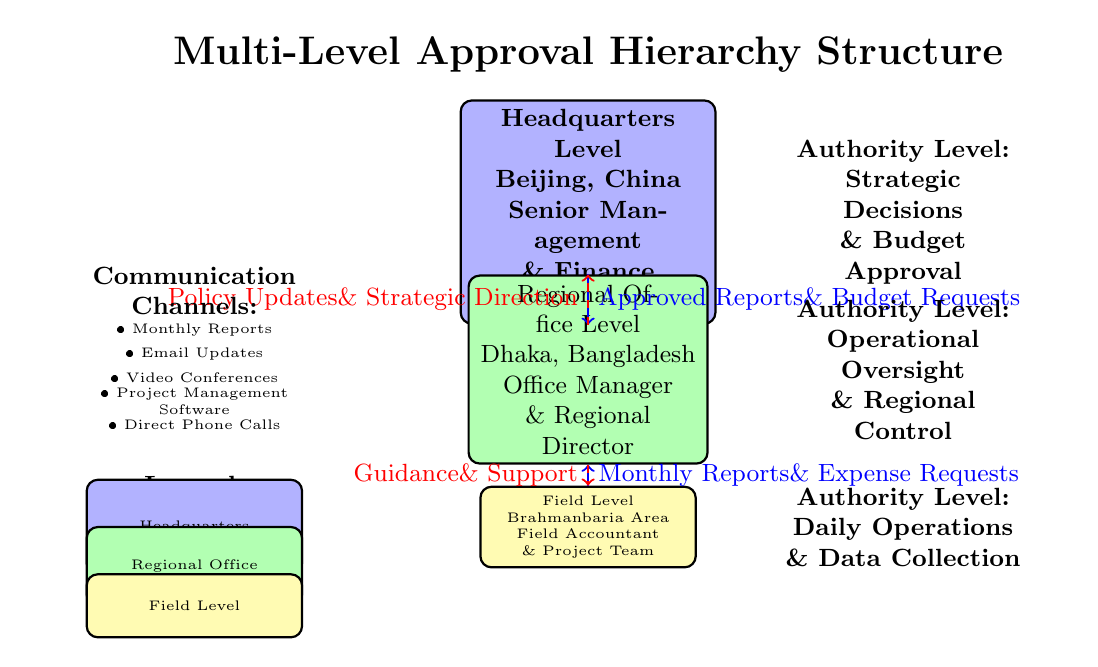
\begin{tikzpicture}[
    node distance=2cm,
    auto,
    thick,
    level 1/.style={rectangle, draw, fill=blue!30, text width=3cm, text centered, rounded corners, minimum height=1.2cm, font=\small\bfseries},
    level 2/.style={rectangle, draw, fill=green!30, text width=2.8cm, text centered, rounded corners, minimum height=1cm, font=\small},
    level 3/.style={rectangle, draw, fill=yellow!30, text width=2.5cm, text centered, rounded corners, minimum height=0.8cm, font=\tiny}
]

% Title
\node[text width=12cm, text centered, font=\Large\bfseries] (title) at (0,8) {Multi-Level Approval Hierarchy Structure};

% Level 1 - Headquarters
\node[level 1] (headquarters) at (0,6) {Headquarters Level\\Beijing, China\\Senior Management\\\& Finance Department};

% Level 2 - Regional Office
\node[level 2] (regional_office) at (0,4) {Regional Office Level\\Dhaka, Bangladesh\\Office Manager\\\& Regional Director};

% Level 3 - Field Level
\node[level 3] (field_accountant) at (0,2) {Field Level\\Brahmanbaria Area\\Field Accountant\\\& Project Team};

% Arrows showing approval flow
\draw[->, thick, blue] (field_accountant) -- node[right, font=\small] {Monthly Reports\\\& Expense Requests} (regional_office);
\draw[->, thick, blue] (regional_office) -- node[right, font=\small] {Approved Reports\\\& Budget Requests} (headquarters);

% Feedback arrows
\draw[->, thick, red, dashed] (headquarters) -- node[left, font=\small] {Policy Updates\\\& Strategic Direction} (regional_office);
\draw[->, thick, red, dashed] (regional_office) -- node[left, font=\small] {Guidance\\\& Support} (field_accountant);

% Authority levels
\node[text width=3cm, text centered, font=\small\bfseries] (authority1) at (4,6) {Authority Level:\\Strategic Decisions\\\& Budget Approval};
\node[text width=3cm, text centered, font=\small\bfseries] (authority2) at (4,4) {Authority Level:\\Operational Oversight\\\& Regional Control};
\node[text width=3cm, text centered, font=\small\bfseries] (authority3) at (4,2) {Authority Level:\\Daily Operations\\\& Data Collection};

% Communication channels
\node[text width=4cm, text centered, font=\small\bfseries] (comm_title) at (-5,5) {Communication Channels:};
\node[text width=4cm, text centered, font=\tiny] (comm1) at (-5,4.5) {• Monthly Reports};
\node[text width=4cm, text centered, font=\tiny] (comm2) at (-5,4.2) {• Email Updates};
\node[text width=4cm, text centered, font=\tiny] (comm3) at (-5,3.9) {• Video Conferences};
\node[text width=4cm, text centered, font=\tiny] (comm4) at (-5,3.6) {• Project Management\\Software};
\node[text width=4cm, text centered, font=\tiny] (comm5) at (-5,3.3) {• Direct Phone Calls};

% Legend
\node[text width=3cm, text centered, font=\small\bfseries] (legend_title) at (-5,2.5) {Legend:};
\node[level 1, text width=2.5cm, font=\tiny] (legend1) at (-5,2) {Headquarters};
\node[level 2, text width=2.5cm, font=\tiny] (legend2) at (-5,1.5) {Regional Office};
\node[level 3, text width=2.5cm, font=\tiny] (legend3) at (-5,1) {Field Level};

\end{tikzpicture}

\end{document}
